\section{System Architecture}
As previously mentioned, there are many layers of abstraction in the program before one actually reaches the hardware level of the sensors. In this section, we will describe these layers, going from the high-level programming of the model, e.g. the architecture described on figure \ref{fig:softwareArchitecture}, down to the hardware specifics of the sensors themselves. 

The intend is, of course, that these software abstractions will not affect our model implementation, aside from the fact that we have to include some libraries to facilitate sensor communication (for instance "ecrobot\_interface.h" and similar). See figure \ref{fig:abstractionLayers} for the system architecture and its layers of abstraction. The dark blue object "Components" consists of all the software inside the components planned in the previous section \ref{fig:softwareArchitecture}. 

\begin{figure}[H]
    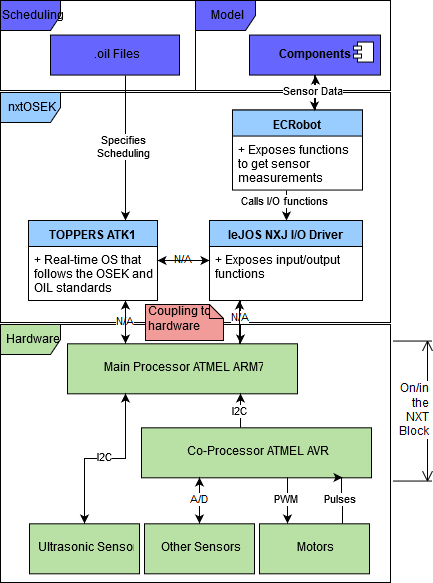
\includegraphics[width=\textwidth]{Images/Design/abstractionLayerDiagram.png}
    \caption{The system architecture of the product, going from high-level programming down to low-level hardware specifics}
    \label{fig:abstractionLayers}
\end{figure}

The note "Coupling to hardware" and the "N/A" edges exists because those are implementation details inside nxtOSEK, which we do not really have access to. In the hardware frame, the edges signify communication protocols such as PWM (pulse width modulation, as described in section \ref{analysisMotors}). 

